\subsection{The interface}
\gls{igro} is a web platform fully developed in R with aid of Shiny libraries, combining the power of the R statistical instrument with HTML5/javascript flexibility.

Shiny apps are typically designed for small applications, allowing a very easy and versatile way for developing and releasing them.
The basic structure of a shiny app is based on two main entities, the \gls{sui} and the \gls{ss}.
The first one includes all the aesthetic components which the user interact with, while the \gls{ss} processes all the computations.

Natively, shiny apps support only one server, but when the needs grow up and multiple interfaces are needed the things become more complicated. 

Our case is composed of a high number of methodologies for multiple-omics problem solving and required a more complex implementation.
To account our problematic, we choose to build \gls{igro} as self-containing modules, by using recently born shiny modules technology \footnote{\url{https://shiny.rstudio.com/articles/modules.html}}.
In such a way, the main shiny app can be shredded in multiple "mini apps", each one with its own \gls{sui} and \gls{ss}.
This approach is totally invisible to the final user but helps the developer for the maintainability and the extensibility of the entire tool.
Indeed, when future needs arise for the implementation of novel functionalities, it is necessary just to implement a novel module.

Our tool presents itself with an upper menu of main topics organized by main scopes. 
For each of these topics, a sub-menu with specific functionalities is available.
When additional functionalities are available, they appear in a left side menu.
In order to well set up the parameters for each functionality, an additional side menu is presented with the parameters and their possible values for the right setup (figure \ref{fig:integrhomain} shows a general representation of the main interface).

\begin{figure}[H]
\centering
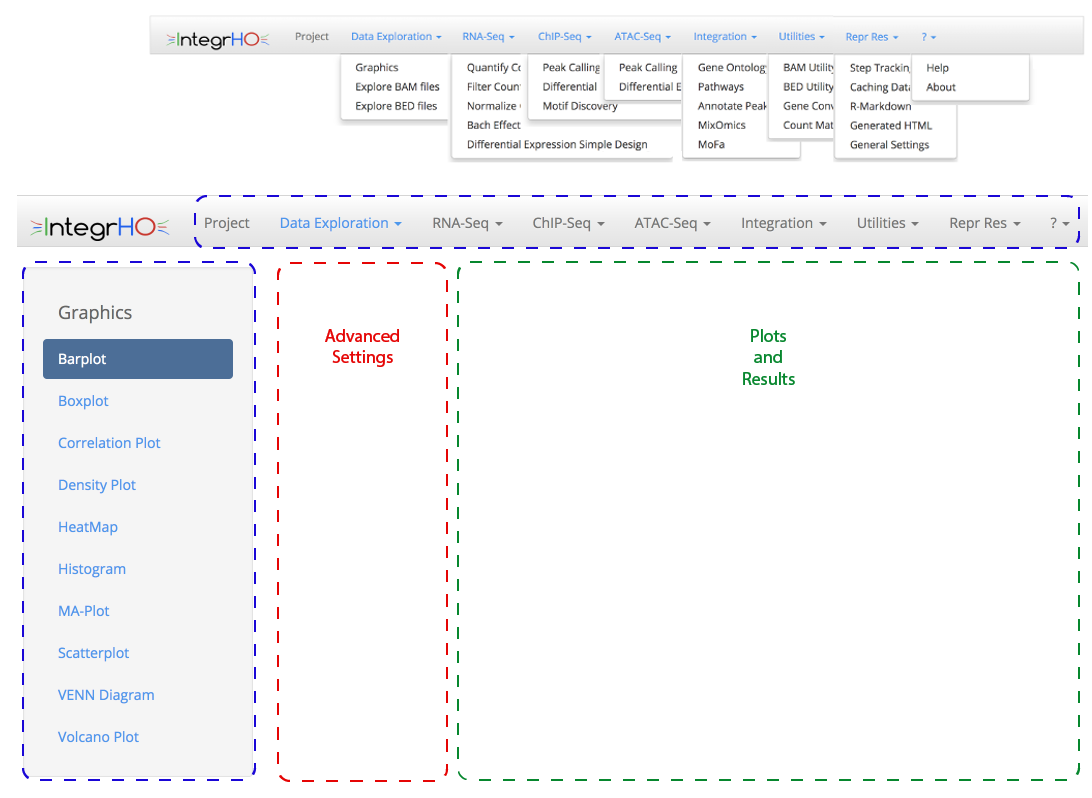
\includegraphics[width=\textwidth, keepaspectratio]{img/integrho/interface.png}
\caption[\gls{igro} main interface]{\gls{igro} main interface description. A main menu in the upper part is presented with all the available main functionalities, and a left side menu is presented with additional functionalities (in blue). Red part indicates the settings for each functionality within the parameter setup. While in green results in table or graphical form are presented.}
\label{fig:integrhomain}
\end{figure}

Once the user set up the required parameters and used the section button the results are shown in graphical or table format in the main part of the interface.

Before to proceed to data analysis, it is mandatory for the user to set up the project with a dedicated interface. 
The user has to upload a design file which describes the information related to its samples, some of them are mandatory as the filename (with path) of the \gls{bam} files and the condition of each sample, while others are optional as the tissue or the run id. 
It is also possible to manually edit the design matrix directly from the interface (figure \ref{fig:integrhodesign}).

The choice of using a mandatory variable describing the path of  \gls{bam} filenames is due to a \textit{Shiny} library limitation. 
Because of its ''ui-server'' structure, shiny applications, when using a \lstinline!fileInput! widget, make a temporary copy of the selected file(s).
But this aspect become really problematic when a file can reach several gigabytes, as a  \gls{bam} file.
Even if there are alternative packages, such as \textit{shinyFiles} \cite{shinyFiles}, offering the possibility to solve the problem, they are not very well tested over multiple platform architectures, bringing us to choice for this workaround solution.


\begin{figure}[H]
\centering
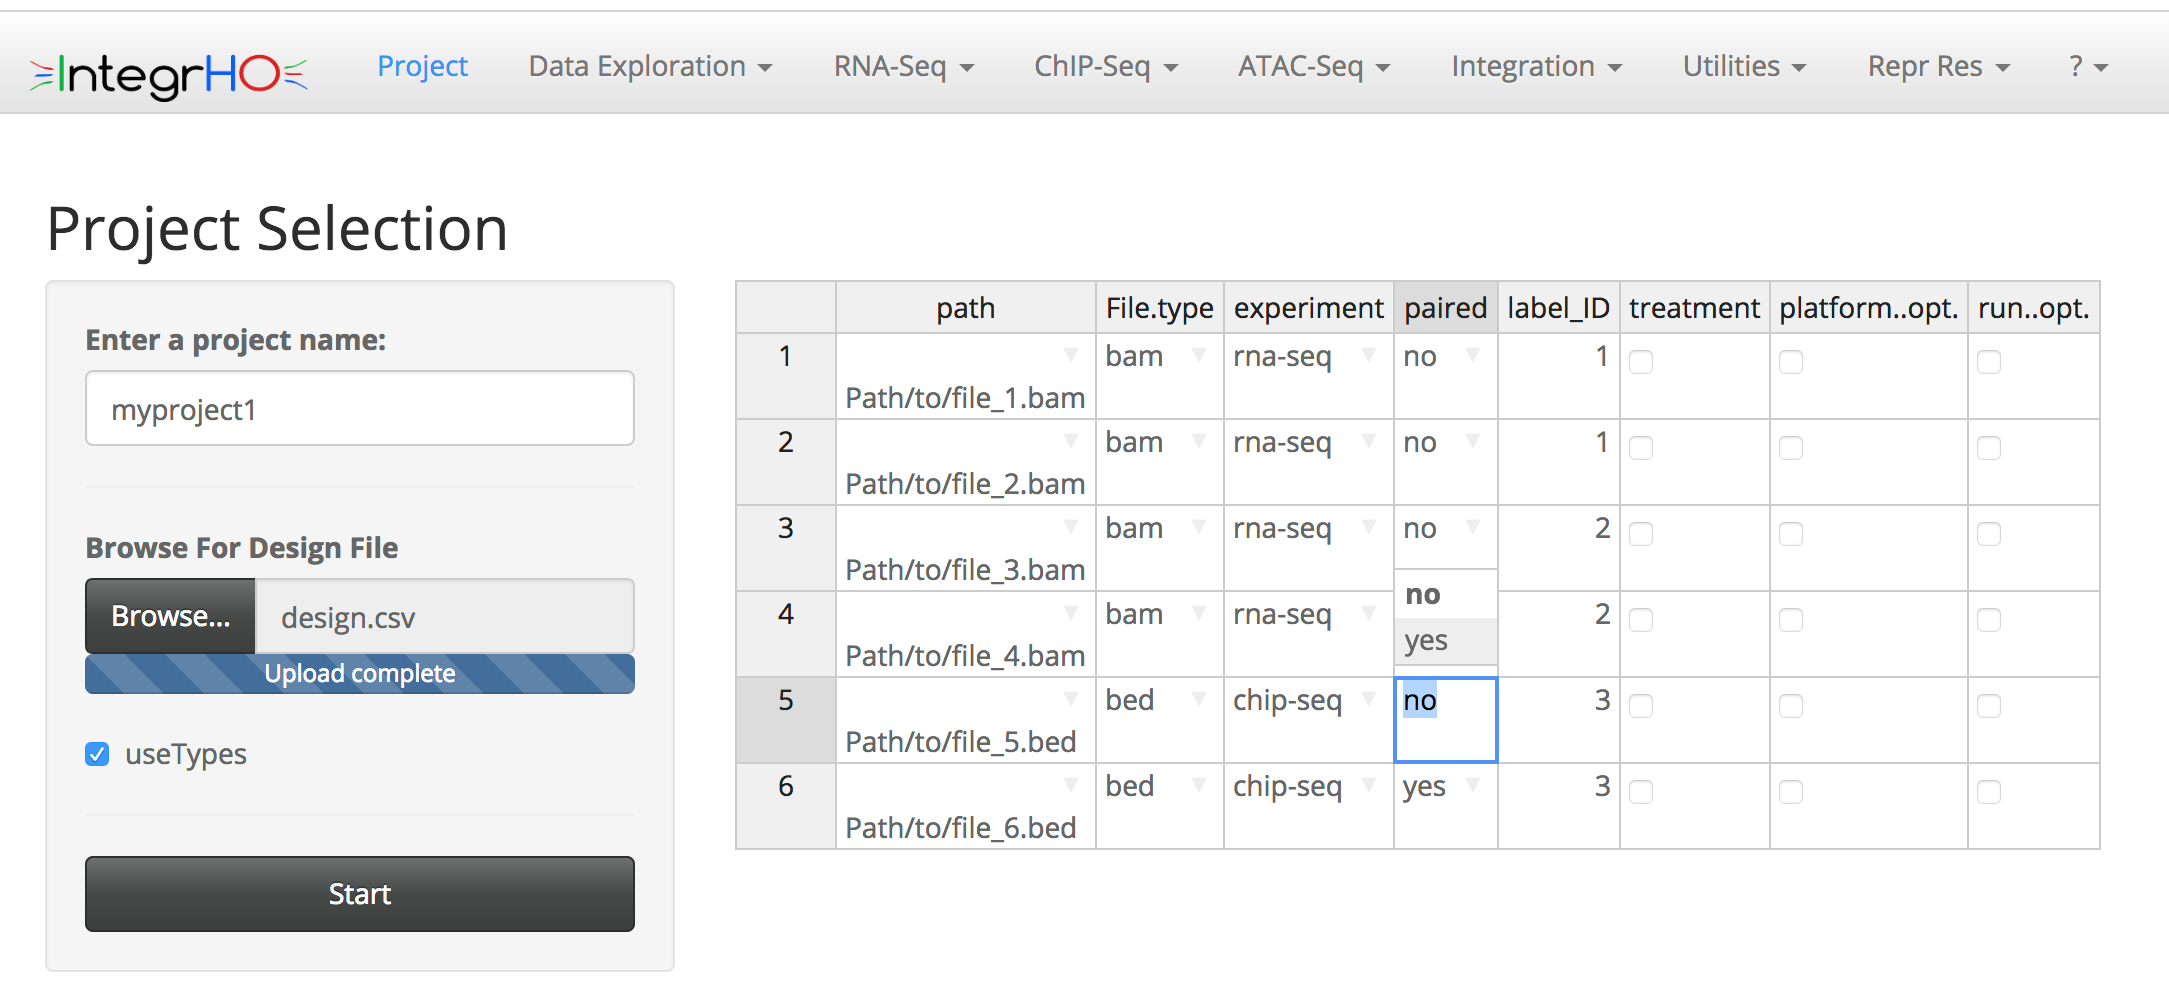
\includegraphics[width=\textwidth, keepaspectratio]{img/integrho/design.png}
\caption[\gls{igro} design interface]{A screenshot of the project design \gls{igro} interface.}
\label{fig:integrhodesign}
\end{figure}

Using the project interface, \gls{igro} creates inside the working directory (returned by the \lstinline!getwd()! function) a dedicated folder with all the required sub-folders and stores all the basic information of the project into an ad-hoc designed \lstinline!R6ProjectClass!, which is re-used during the whole session to speed up the configuration of each step of the analysis (Figure \ref{fig:integrhotree} shows a representation of a typical folder tree produced for a project).

\begin{figure}[H]
\centering
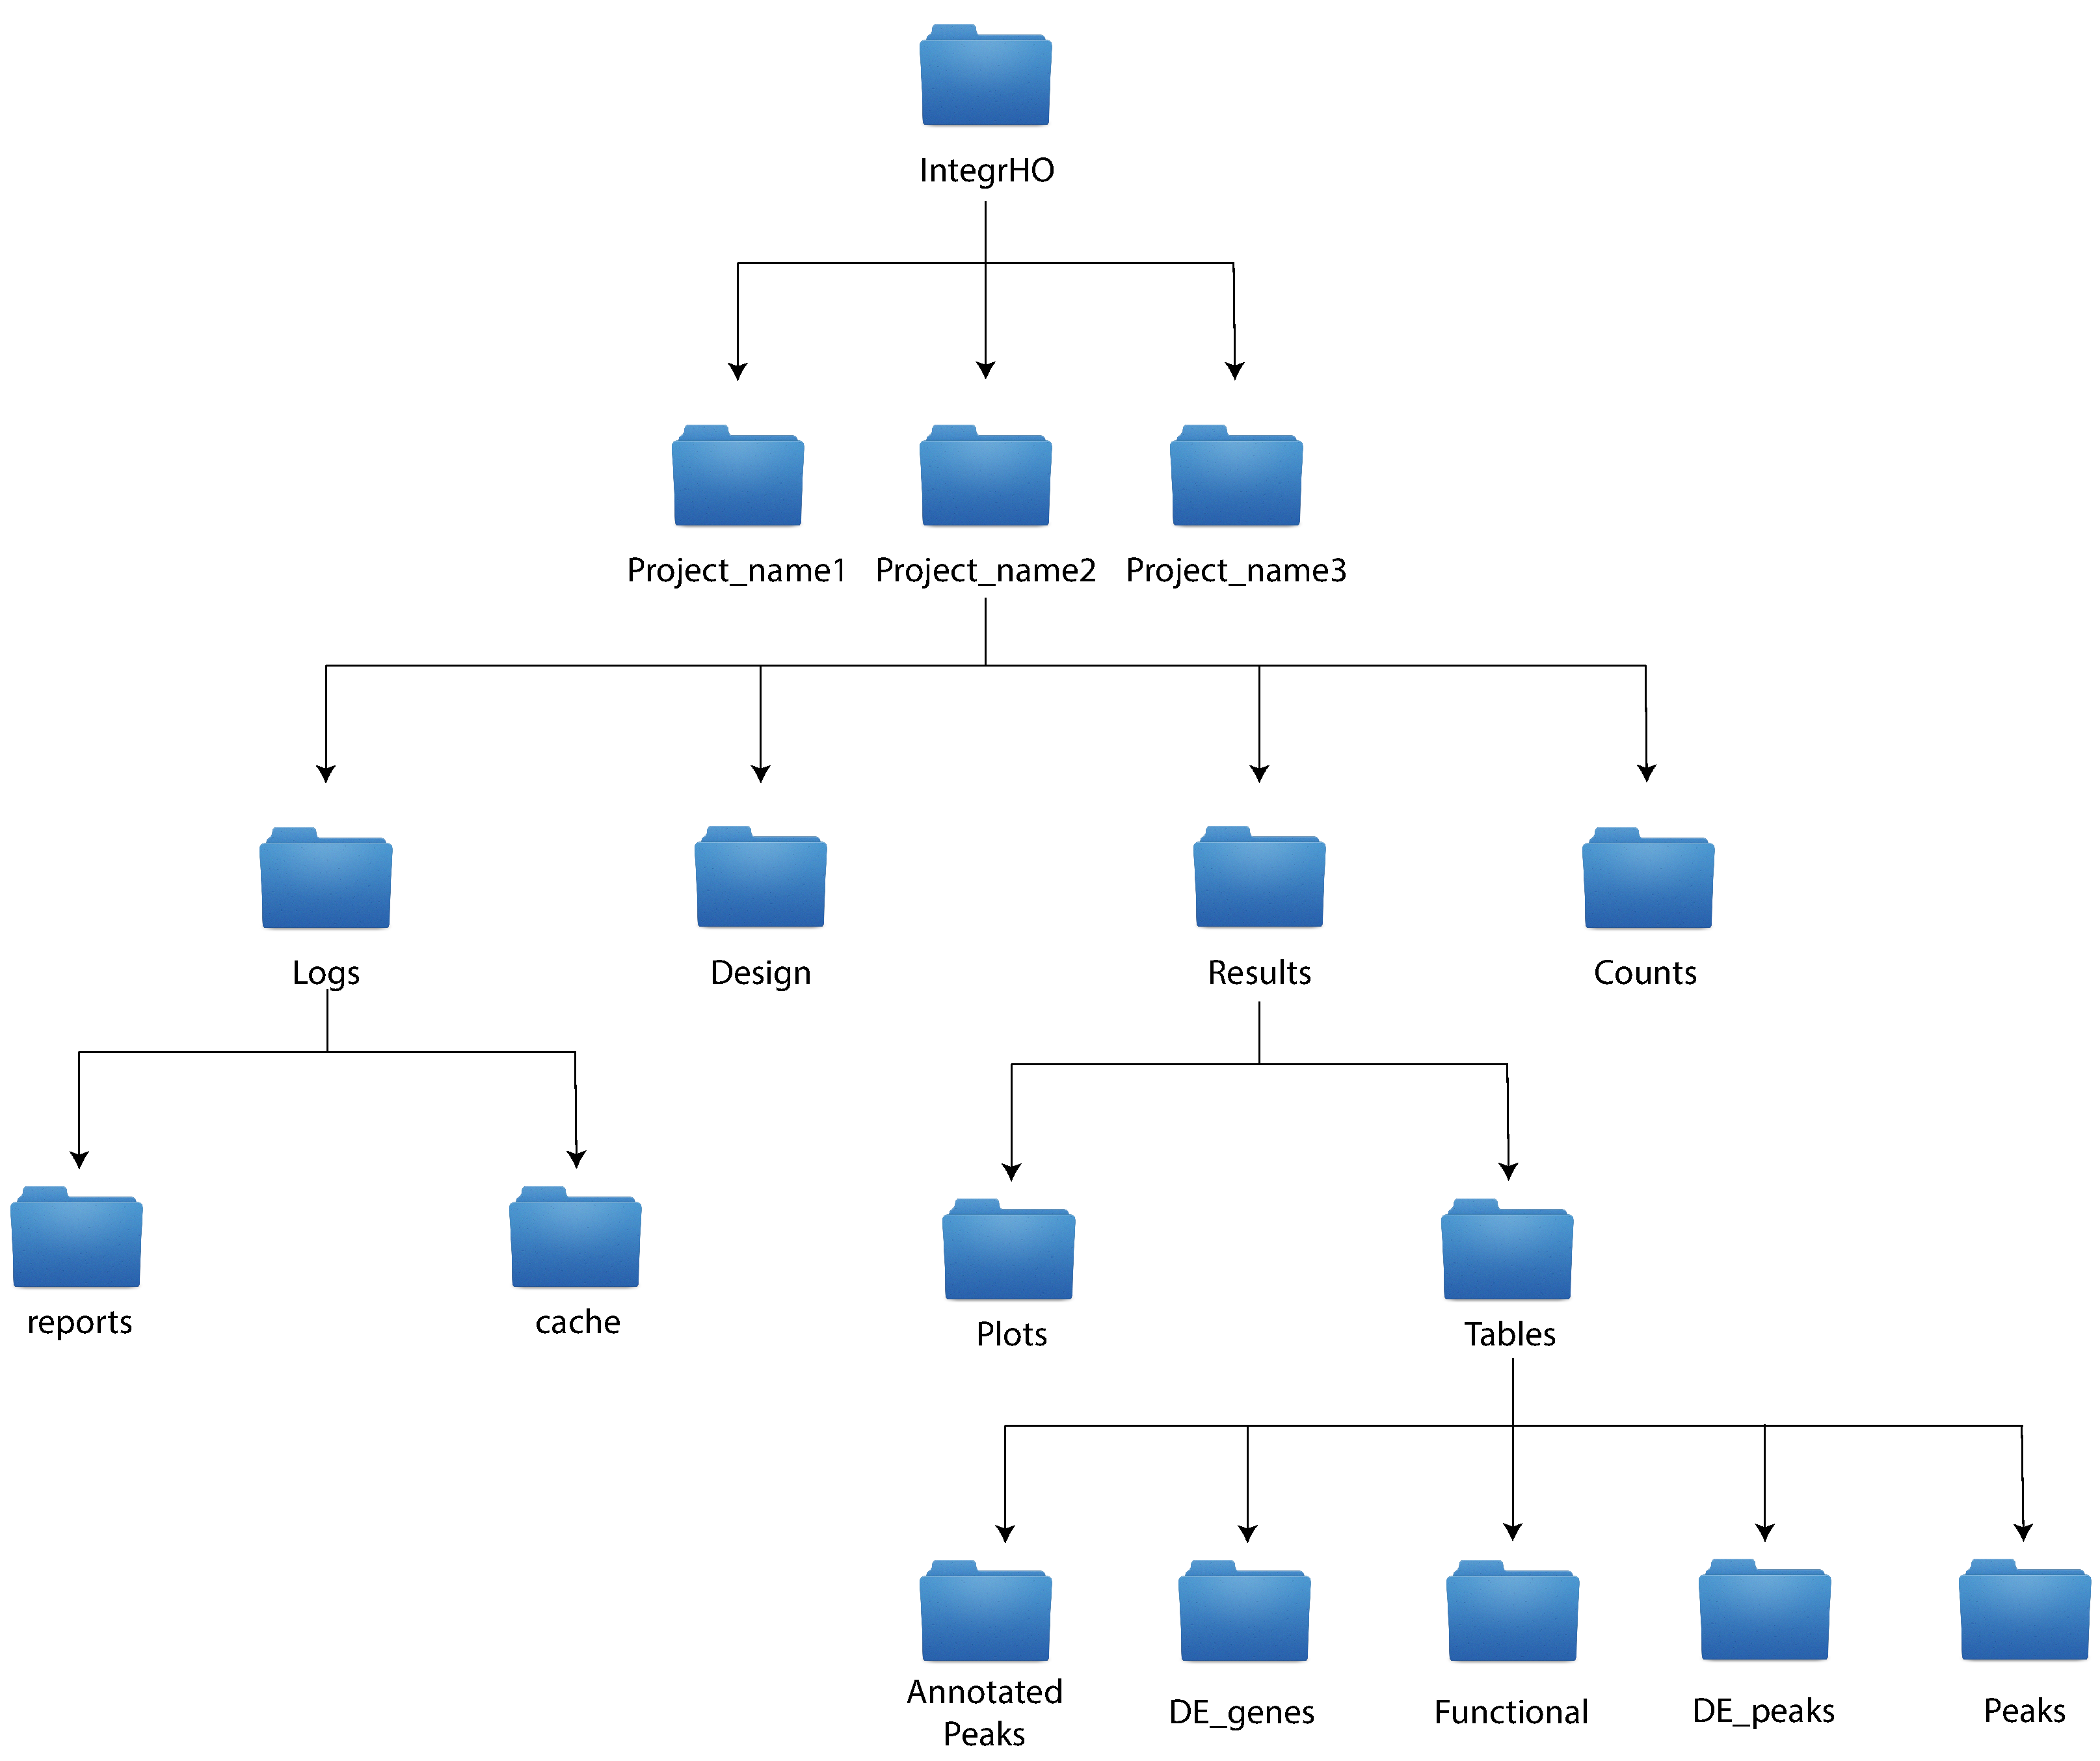
\includegraphics[width=\textwidth, keepaspectratio]{img/integrho/project_folder.pdf}
\caption[\gls{igro} folder tree]{A schematical representation of \gls{igro} project folder tree.}
\label{fig:integrhotree}
\end{figure}

In particular, the \lstinline!R6ProjectClass! stores all the paths represented inside the figure \ref{fig:integrhotree}, giving fast access to the files stored in each folder, when an interface is selected.


\subsection{Available Methodologies}

Unlike tools as Galaxy \cite{Hillman-Jackson2012} and Taverna \cite{Wolstencroft2013}, focused on analysis workflows, \gls{igro} gives to the user high freedom of interaction, reporting all performed steps in a human-readable \textit{HTML} report.
 
Actually, \gls{igro} methodologies can be organized have been organized in a way that the user can analyze each single omics, and afterwards combine the results to obtain an integrated view of them (figure \ref{fig:integrhoidea} shows a schematic representation of \gls{igro}).

In particular, we defined specific interfaces for \textit{RNA-seq}, \textit{ChIP-seq} and \textit{ATAC-seq} data, providing additional interfaces for their integration, such as \textit{functional enrichment} and \textit{gene-peak} annotations.
%It implements not only the methodologies reported inside \textit{ticorser} for \textit{RNA-Seq} and \textit{DEScan2} for \textit{ATAC-Seq}, but implements also methodologies for \textit{ChIP-Seq} data analysis, complementing these aspects by providing functionalities for their integration at different levels, such as functional enrichment with Gene Ontology and Pathways and peaks-genes annotation.

\begin{figure}[H]
\centering
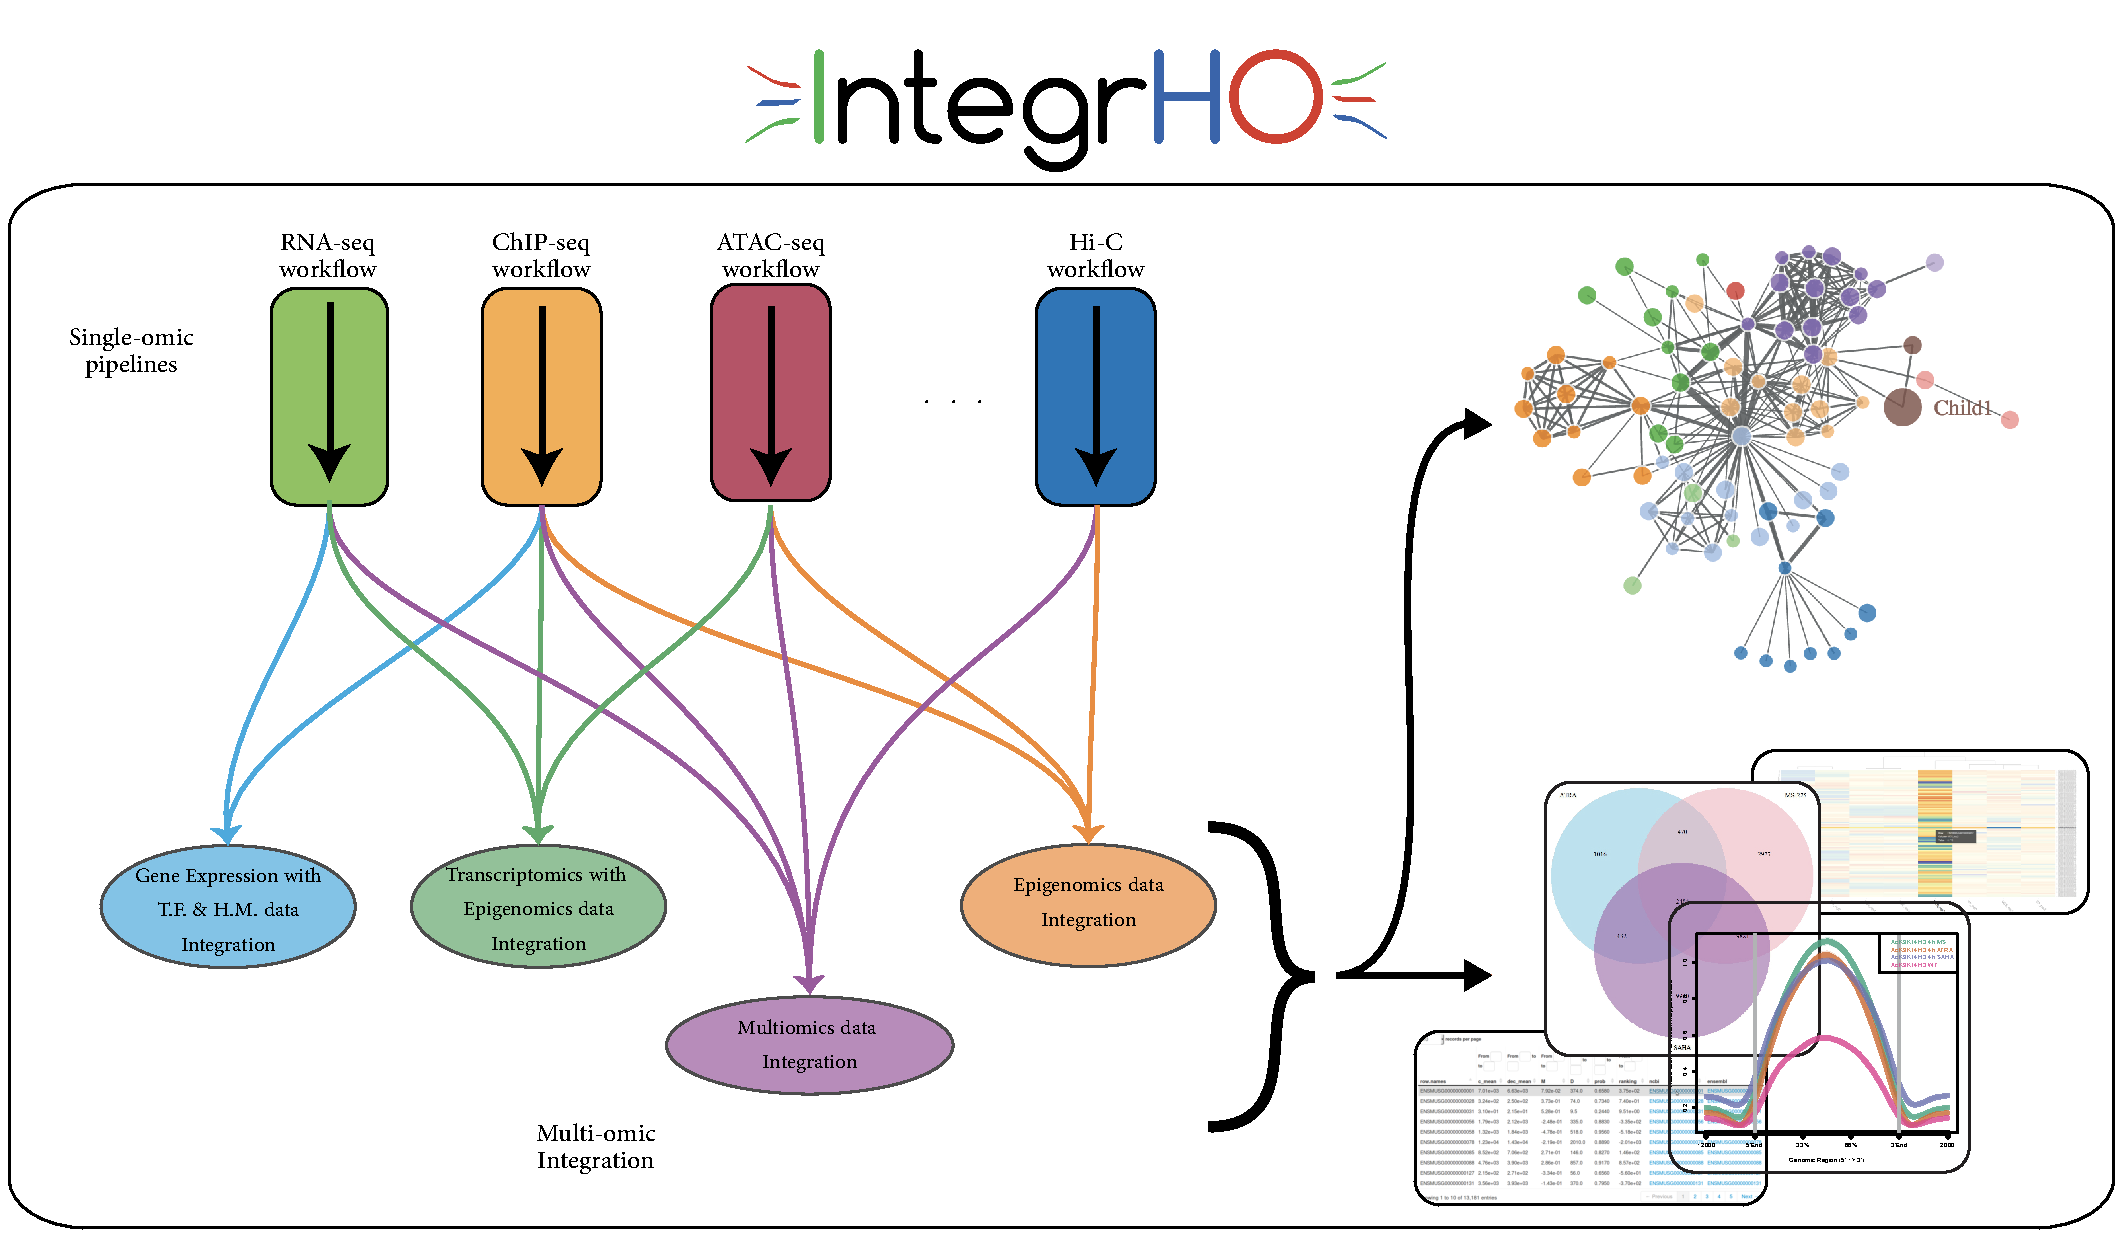
\includegraphics[width=\textwidth, keepaspectratio]{img/integrho/integrho_scheme.pdf}
\caption[\gls{igro} representation]{A schematical representation of \gls{igro} underlying idea.}
\label{fig:integrhoidea}
\end{figure}

%\subsubsection{Graphics}
\subsubsection{RNA-seq}
For \textit{RNA-seq} we chose multiples methods for allowing the user to obtain an good overview of this omics analysis.


{\setlength{\parindent}{0cm}\textbf{Features Quantification}}

When selecting the \lstinline!Quantify Counts! an interface designed for \lstinline!featureCounts! of \lstinline!Rsubread! R/Bioc package function \cite{Liao2014} appears.
The  \gls{bam} file paths for the \textit{RNA-seq} data are automatically selected from the   design matrix loaded during the project creation phase.

We choose proper widgets for selecting the reference genome and its annotation, it is also possible to configure the \lstinline!featureType! to use, while the \lstinline!attributeType! is set by default to \lstinline!gene_id!.
Additionally parameters can be selected for \lstinline!allowMultiOverlap! and to select if the reads are \lstinline!paired!.
Finally, the number of thread to use can be set from 1 to 8.

At the end of the processing the resulting count matrix is presented in the main part of the interface as a \lstinline!data.table! format, and automatically stored inside the \lstinline!IntegrHO/project_name/counts! folder.


{\setlength{\parindent}{0cm}\textbf{Counts Filtering and Normalization}}

When selecting the \lstinline!Filter Counts! the designed interface automatically loads the counts files inside the \lstinline!IntegrHO/project_name/counts!, otherwise allowing, with a \lstinline!fileInput! widget, to chose another count matrix file.
It is possible to switch between three different filtering methods (\textit{Proportion Test}, \textit{Wilcoxon Test}, \textit{CPM}), as defined inside the \lstinline!filtered.data! function of \textit{NOISeq} R/Bioconductor package \cite{Tarazona2012}.

The same type of interface is loaded when the \lstinline!Normalize Counts! menu voice is selected.
Three different normalization methods can be selected, the \textit{Trimmed Mean of M-values} \cite{Robinson2010}, the \textit{Upper Quartile} and the \textit{Full Quantile}.

When selecting the \lstinline!Batch Effect! section there will be the possibility to apply the \textit{RUVs} or \textit{RUVg} methods from \textit{RUVSeq} R/Bioconductor package \cite{Risso2014h}.
Moreover, when selecting one of this methods, an additional file can be loaded, in order to upload an optional list of negative control genes.

To graphically inspect the normalized data two different plots will be presented into the main interface, the \gls{pca} and the \textit{boxplots} for before and after normalization of the samples.

Finally, at the end of execution the filtered/normalized features, as \gls{tsv} file format, are stored inside the \lstinline!IntegrHO/project_name/counts! folder, adding at the end of the file name the ''transformation'' applied.


{\setlength{\parindent}{0cm}\textbf{Differential Expression Methods}}

In order to detect \glspl{deg}, we designed the \lstinline!Differential Expression Simple Design!, where it is possible to choose between four different methods.

The available count matrix files are automatically loaded from the \lstinline!IntegrHO/project_name/counts! folder.
Otherwise, the user can additionally load another count matrix file using the apposite file selector.

In order to address for the factors to analyze, the interface automatically gives the possibility to select the design matrix column name where to fine them.
Additionally, two \lstinline!selectInput! widgets appears where to select the two factors to contrast.

We selected four different methods implemented inside \textit{edgeR}, \textit{DESeq2}, \textit{NOISeq} and \textit{NOISeqBio} R/Bioconductor packages \cite{Robinson2009, Love2014,Tarazona2012}.

In case of \textit{edgeR} we decided to use the \textit{Quasi-Likelihood} method for the differential expression.
While when using \textit{DESeq2} for this specific case we choose the \textit{Wald} test, as the authors suggest.
The \textit{NOISeq} package offers the possibility to discriminate between \textit{biological} and \textit{technical} replicates, computing a posterior probability in both cases, but applying different hypothesis tests.

The dedicated interface automatically shows a \lstinline!tabsetPanel! of 3 different tabs, within, respectively, a \textit{VolcanoPlot}, an \textit{MA-Plot} and the table of the \gls{deg} results.


\subsubsection{ChIP-seq}

For \textit{ChIP-Seq} we constructed specific interfaces for peak calling and \glspl{der} detection.

{\setlength{\parindent}{0cm}\textbf{Peak Calling}}

For the peak calling, because of the lack of specific methods starting from \gls{bam} files in R, we implemented a dedicated interface for \textit{csaw} \cite{Lun2015} peak caller, which allows quantification for both broad and narrow peaks, typically resulting from \gls{hm} and \gls{tf} \textit{ChIP-seq} data.

Firstly, it is possible to select the design matrix (stored inside \lstinline!IntegrHO/project_name/design! folder) and the column specifying the experiment.
In such a way, \gls{igro} is able to pick up the \gls{bam} filenames associated to the \textit{CHiP-seq} experiments by itself.

Afterwards, the interface enables the specification of several parameters useful for the \lstinline!windowCounts! method of \textit{csaw} R/Bioconductor package.
The method constructs a count matrix where the rows indicate the detected windows of length \lstinline!window width!, and the columns indicate samples.

Additional parameters selected for the analysis with the \textit{csaw} method are the \lstinline!paired end reads!, a flag for ignoring duplicated reads with \lstinline!ignore duplicates!, and the possibility to make the analysis only on a list of chromosomes, using \lstinline!chromosomes list! implemented with a \lstinline!selectizeInput!.
The possibility to make parallel computing is implemented with \lstinline!core number! widget.

At the end of the processing the count matrix is shown into the main part of the interface, and it is saved as \gls{tsv} format, into the \lstinline!IntegrHO/project_name/results/tables/peaks! folder.
In order to distinguish the produced output from others, the results file is saved adding the method name at the end of the filename.

{\setlength{\parindent}{0cm}\textbf{Differential Binding}}

Thanks to the counts matrix form, we are able to apply the same methodologies designed for \textit{RNA-seq} data.
For this reason we used the same  methods as defined for \textit{RNA-seq}, with a main difference on the output.

In this case the output module is by a the \glspl{dbs} table


\subsubsection{ATAC-seq}

Thanks to the work made with \gls{descan} (chapter \ref{sec:descan2cap}), we had the possibility to deeply investigate \textit{ATAC-seq} data, presenting a specific analysis workflow.

We tried to give access to the same methodologies here in \gls{igro}, in order to simplify and spread the proposed work.


{\setlength{\parindent}{0cm}\textbf{Region Detection}}

In particular we built a specific interface for the peak caller (see section \ref{sec:descan2peakcall}) defined in \gls{descan}.

As for the \textit{csaw}, the user can select the design matrix (stored inside \lstinline!IntegrHO/project_name/design! folder) and the column associated to the experiment definition.
Additional parameter selection is required for the selection of the \lstinline!genome name!, the \lstinline!bin size! for the genome binning, and for the \lstinline!max window! and \lstinline!min window! lengths.
Also in this case we gave the possibility to select for a multi-core computation with the \lstinline!core number! sliderInput widget.

The user can also select the \lstinline!peak score! threshold for filtering out the regions with lower score than the threshold, and the \lstinline!samples threshold! for the alignment phase (see section \ref{descan2filtering}).

In order to better compare \gls{descan} results with similar methods, such as \textit{casw}, we preferred to include also the \gls{descan} filtering method inside the \textit{region detection} interface.
In such a way, the presented output is a count matrix of detected regions on the rows and samples on the columns.

{\setlength{\parindent}{0cm}\textbf{Normalization}}



For the annotation we selected the \textit{ChIPpeakAnno} and the \textit{ChIPseeker} R/Bioconductor packages, which produces similar output formats starting from peaks.
While for the detection of \glspl{der} we used the same methods as for \textit{RNA-seq}.

For \textit{ATAC-seq} we used mostly the same methods implemented for the \textit{ChIP-Seq}, but designing specific interfaces for the filtering/alignment and the counting matrix as implemented in the \textit{DEScan2} package (see chapter \ref{sec:descan2cap} for further details).

To provide an integration of these omics, we dedicated an entire section to this aspect, with functionalities for the annotation of \glspl{der} with \glspl{deg} using \textit{ChIPpeakAnno} and to use this information to investigate the functional response by enrichment for Gene Ontology or for Pathways.
These last two aspects implemented with aid of \textit{g:Profiler} \cite{Reimand2016} and \textit{graphite} \cite{Sales2012a} R/Bioconductor packages.


For each -omics, \gls{igro} takes as input \gls{bam} files, previously defined inside the design matrix of the main project definition interface.

Moreover, not only our software offers lots of utilities for data management and analysis, but also a great variability of graphics, useful to explore data and results, both in pre-processing and post-processing phase, such as \textit{barplots}, \textit{correlation plots}, \textit{heatmap}, \textit{scatterplots}, etc.

In order to facilitate the multi-omic data integration, we assembled several R functions to be freely combined in order to analyse each single-omic data type and to use their results for multi-omic data integration (Figure 1).